% \documentclass{beamer}
% \usetheme{metropolis}           % Use metropolis theme
% \title{Visual assessments of Postural
% Orientation Errors using
% ensembles of Deep Neural
% Networks}
% \date{\today}
% \author{Filip Kronström}
% \institute{Lund University}
% \begin{document}
%   \maketitle
%   \section{First Section}
%   \begin{frame}{First Frame}
%     Hello, world!
%   \end{frame}
% \end{document}

\documentclass[10pt]{beamer}

\usetheme{metropolis}
\usepackage{appendixnumberbeamer}
% \usepackage{setspace}

\usepackage{booktabs}
\usepackage[scale=2]{ccicons}
% \usepackage{footmisc}
\usepackage{scrextend}
% \usepackage{setspace}
\usepackage{pgfplots}
% \usepackage{multimedia}
\usepackage{animate}
\usepgfplotslibrary{dateplot}
% \addbibresource{files/bibtex/pres_bib.bib}

% \setsansfont{Ubuntu}
% \setmonofont{Ubuntu Mono}
\usepackage{tabu}

\usepackage{xspace}
% \usepackage{subcaption}
\newcommand{\themename}{\textbf{\textsc{metropolis}}\xspace}
% \renewcommand{\small}{\footnotesize}
\renewcommand{\footnotesize}{\tiny}
\title{Visual assessments of\\Postural
Orientation\\Errors using
ensembles\\of Deep Neural
Networks}
\subtitle{Master's Thesis}
\date{\today}
\author[me]{\textbf{\large Filip Kronström}\\[1.5mm]Supervisors: A. Jakobsson\footnote{Centre for Mathematical Sciences, Mathematical Statistics, Lund University}, J. Älmqvist\footnote{\label{hs}Department of Health Sciences, Lund University}, E. Ageberg$^{\ref{hs}}$, M. Creaby\footnote{School of Exercise Science, Australian Catholic University \newline}}
\institute{\large Faculty of Engineering, Lund University}
\titlegraphic{\hfill
\includegraphics[height=2.6cm]{files/figs/presentation/lth_logo_en.eps}}

\begin{document}

\maketitle
% \footnotetext[4]{\newline}

\begin{frame}{Agenda}
  \setbeamertemplate{section in toc}[sections numbered]
  \tableofcontents[hideallsubsections]
\end{frame}

\section{Introduction}
% \begin{frame}[fragile]{Sports injuries}
%   % lol\footnote{LaBella et al., Anterior Cruciate Ligament Injuries: Diagnosis, Treatment, and Prevention. 2014}
%     \begin{columns}[T,onlytextwidth]
%       \column{0.45\textwidth}
%         {\small50\% of amateur football players in Denmark experience hip/groin pain during season\footnotemark.}
%       \column{0.45\textwidth}
%         {\small Around 8000 yearly Anterior cruciate ligament injuries in Sweden\footnotemark.}
%     \end{columns}
%     \begin{figure}
%       \centering
%       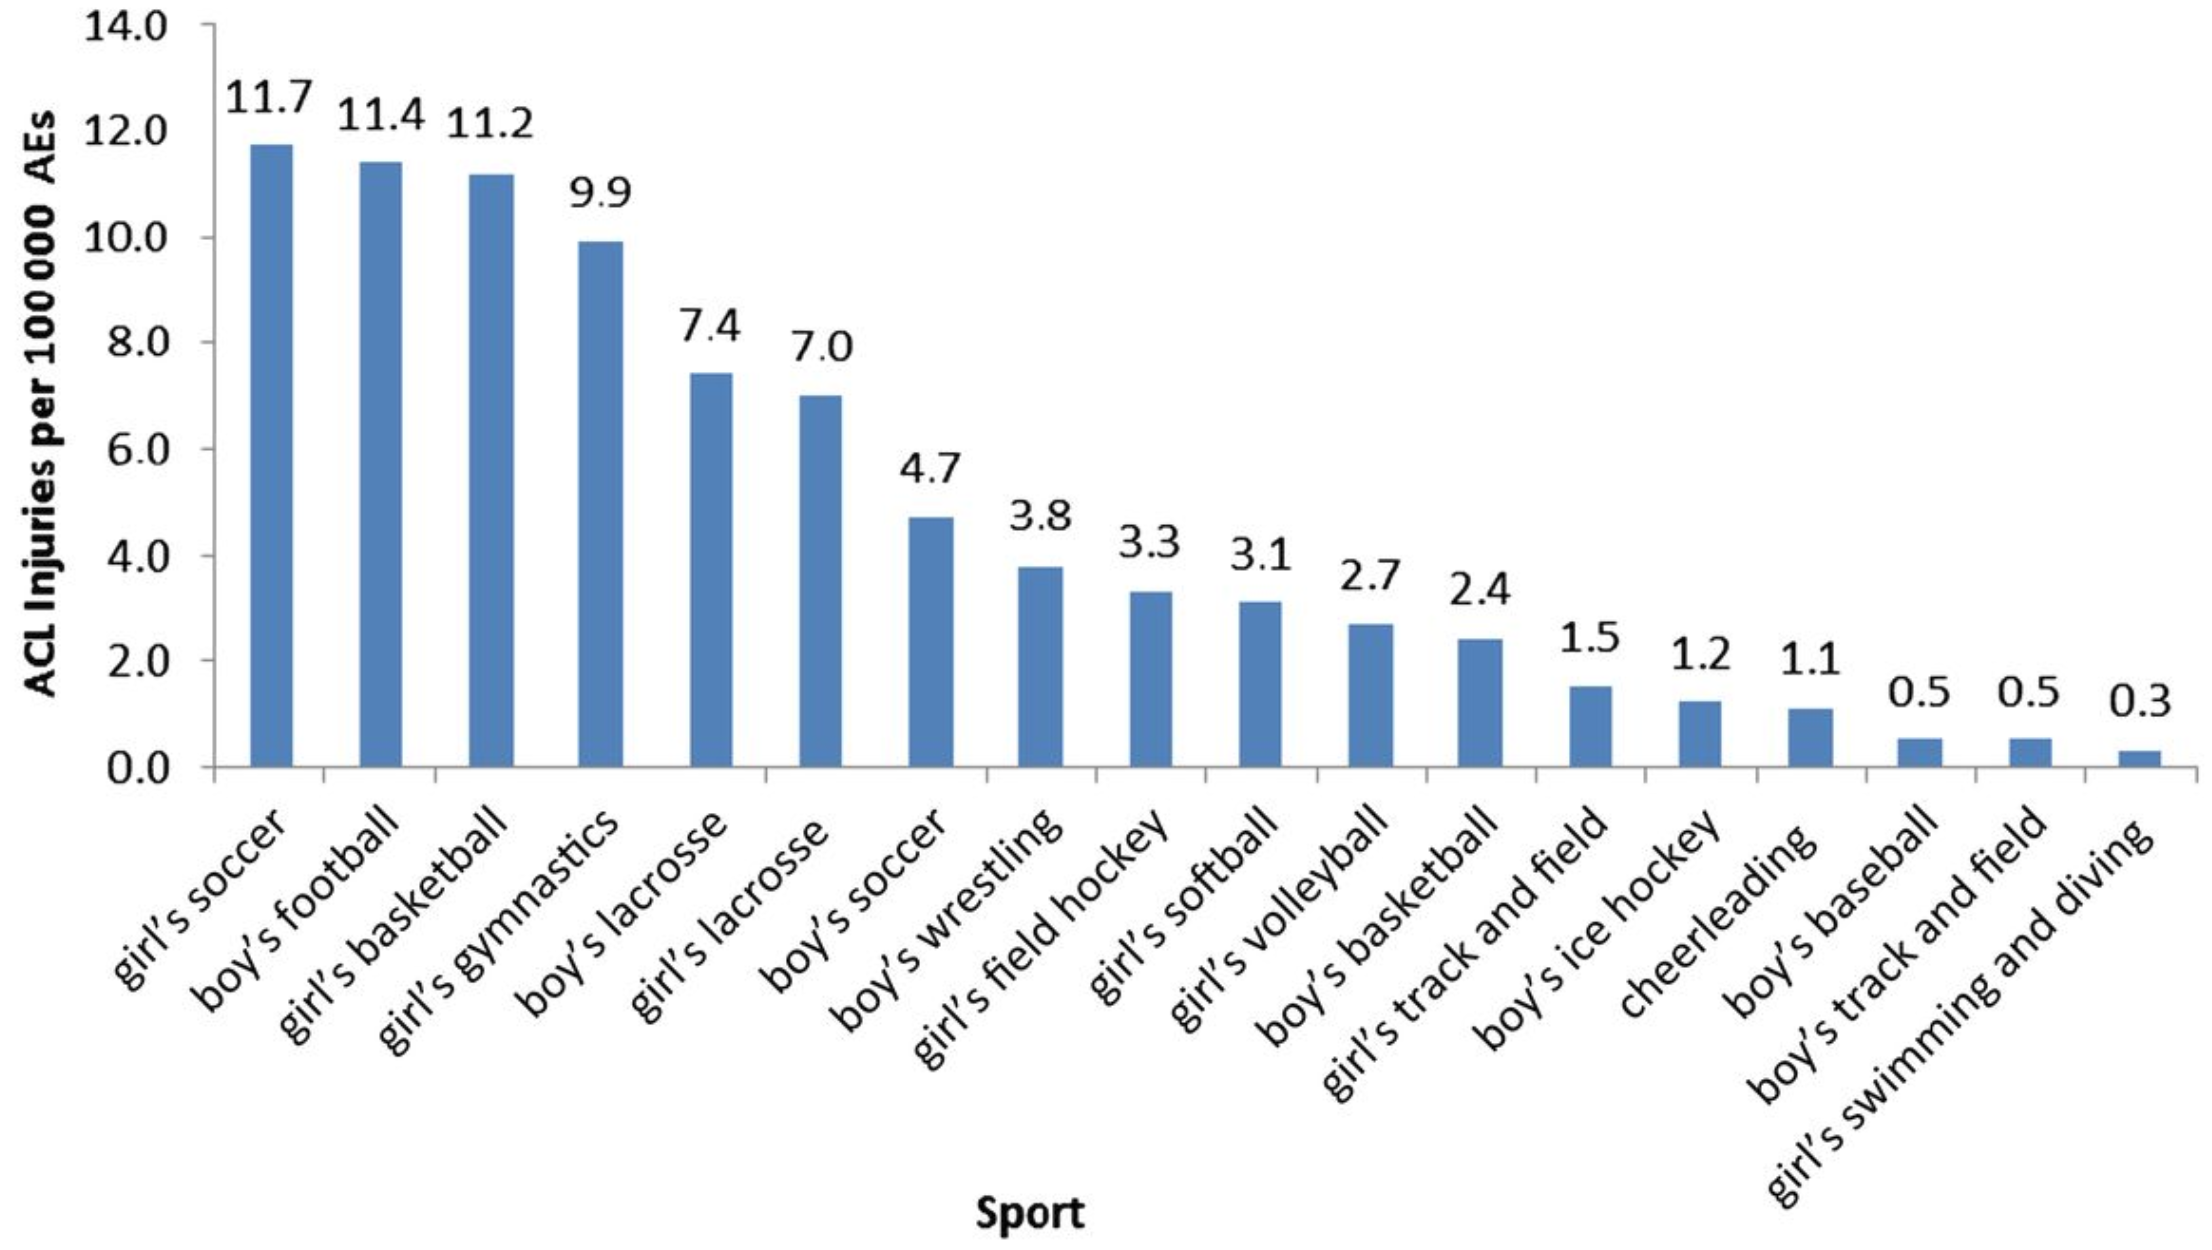
\includegraphics[width=0.75\textwidth]{files/figs/presentation/acl-injury-per-ae.png}
%       % \caption[Caption for LOF]{Injury rates among high school students, per 100 000 athlete exposures\footnote{LaBella et al., Anterior Cruciate Ligament Injuries: Diagnosis, Treatment, and Prevention. 2014}.}
%
%       {\scriptsize\textbf{Figure 1:} Injury rates among high school students, per 100 000 athlete exposures\footnotemark.}
%       % \label{}
%     \end{figure}
%
%
% \footnotetext[1]{Thorborg et al., Prevalence
% and severity of hip and groin pain in sub-elite male football: a cross-sectional cohort study of 695 players. 2017}
% \footnotetext[2]{Svenska korsbandsregistret, Årsrapport 2019. 2020}
% \footnotetext[3]{LaBella et al., Anterior Cruciate Ligament Injuries: Diagnosis, Treatment, and Prevention. 2014}
%
% \end{frame}

\begin{frame}[fragile]{Anterior Cruciate Ligament injuries}
  \begin{columns}[c,onlytextwidth]
    \column{0.53\textwidth}
      \begin{itemize}
        % \small
          \item Around 8000 yearly Anterior cruciate ligament injuries in Sweden.
          \item Regular injury mechanism is sudden changes in direction or velocity while knee is bearing weight.
          \item Rehabilitation typically up to 2 years.
          \item Increased long and short term risk of, e.g., osteoarthritis, joint instability, and re-injury.
      \end{itemize}

    \column{0.52\textwidth}
    \begin{figure}
      \centering
      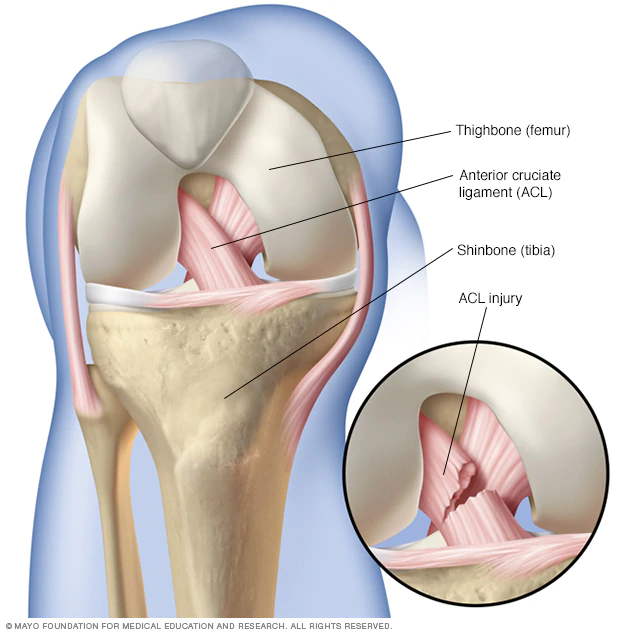
\includegraphics[width=\textwidth]{files/figs/intro/acl.png}
      % \caption{}
      % \label{}

      {\scriptsize\textbf{Figure 1:} Illustration of ACL in the knee\footnotemark.}
    \end{figure}

  \end{columns}

  \footnotetext[1]{Mayo Clinic, \url{https://www.mayoclinic.org/diseases-conditions/acl-injury/symptoms-causes/syc-20350738}}
\end{frame}

% \begin{frame}[c,fragile]{Anterior cruciate ligament injury and rehabilitation}
%   \begin{columns}[c,onlytextwidth]
%     \column{0.45\textwidth}
%       \begin{itemize}
%         % \small
%           \item Regular injury mechanism is sudden changes in direction or velocity while knee is bearing weight\footnotemark.
%           \item Rehabilitation typically up to 2 years\footnotemark.
%           \item Increased long and short term risk of, e.g., osteoarthritis\footnotemark, joint instability\footnotemark, and re-injury\footnotemark.
%       \end{itemize}
%
%     \column{0.55\textwidth}
%     \begin{figure}
%       \centering
%       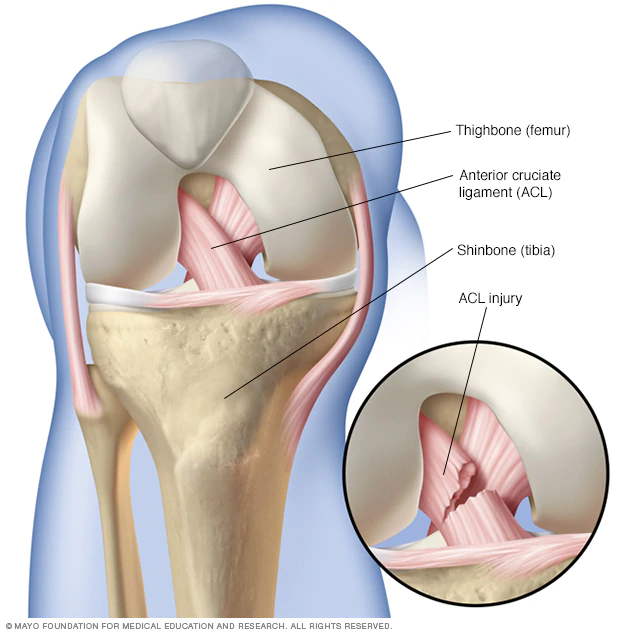
\includegraphics[width=0.9\textwidth]{files/figs/intro/acl.png}
%       % \caption{}
%       % \label{}
%
%       {\scriptsize\textbf{Figure 2:} Illustration of ACL in the knee\footnotemark.}
%     \end{figure}
%
%   \end{columns}
%
%   \footnotetext[4]{Wetters et al., Mechanism of Injury and Risk Factors for Anterior Cruciate Ligament Injury. 2016}
%   \footnotetext[5]{Nagelli and Hewett, Should Return to Sport be Delayed Until 2 Years After Anterior Cruciate Ligament Reconstruction? Biological and Functional Considerations. 2017}
%   \footnotetext[6]{Mayo Clinic, \url{https://www.mayoclinic.org/diseases-conditions/acl-injury/symptoms-causes/syc-20350738}}
%   \footnotetext[7]{Wetters et al., Mechanism of Injury and Risk Factors for Anterior Cruciate Ligament Injury. 2016}
%   \footnotetext[8]{Nagelli and Hewett, Should Return to Sport be Delayed Until 2 Years After Anterior Cruciate Ligament Reconstruction? Biological and Functional Considerations. 2017}
%   \footnotetext[9]{Mayo Clinic, \url{https://www.mayoclinic.org/diseases-conditions/acl-injury/symptoms-causes/syc-20350738}}
%
% \end{frame}

\begin{frame}[fragile]{Postural Orientation}
  \begin{columns}[T,onlytextwidth]
    \centering
    \column{0.55\textwidth}
  \begin{columns}[T,onlytextwidth]
      \column{0.49\textwidth}

      \begin{figure}
        \raggedleft
        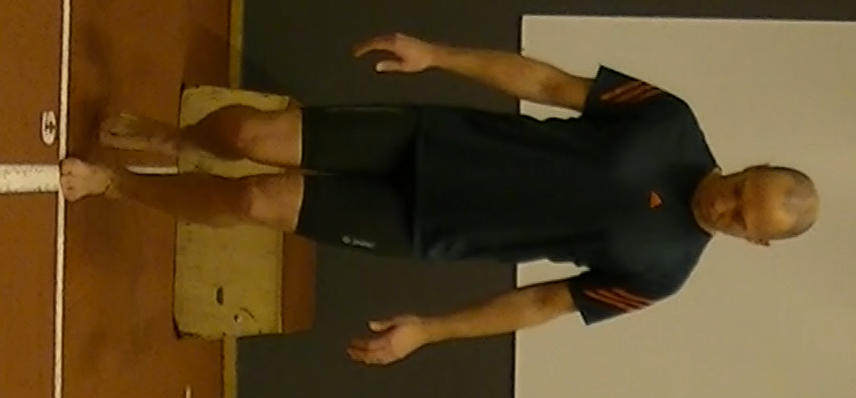
\includegraphics[angle=90,height=0.7\textheight]{files/figs/presentation/good-poe.png}
        % \caption{}
        % \label{}
      \end{figure}

      \column{0.49\textwidth}
      \begin{figure}
        \raggedright
        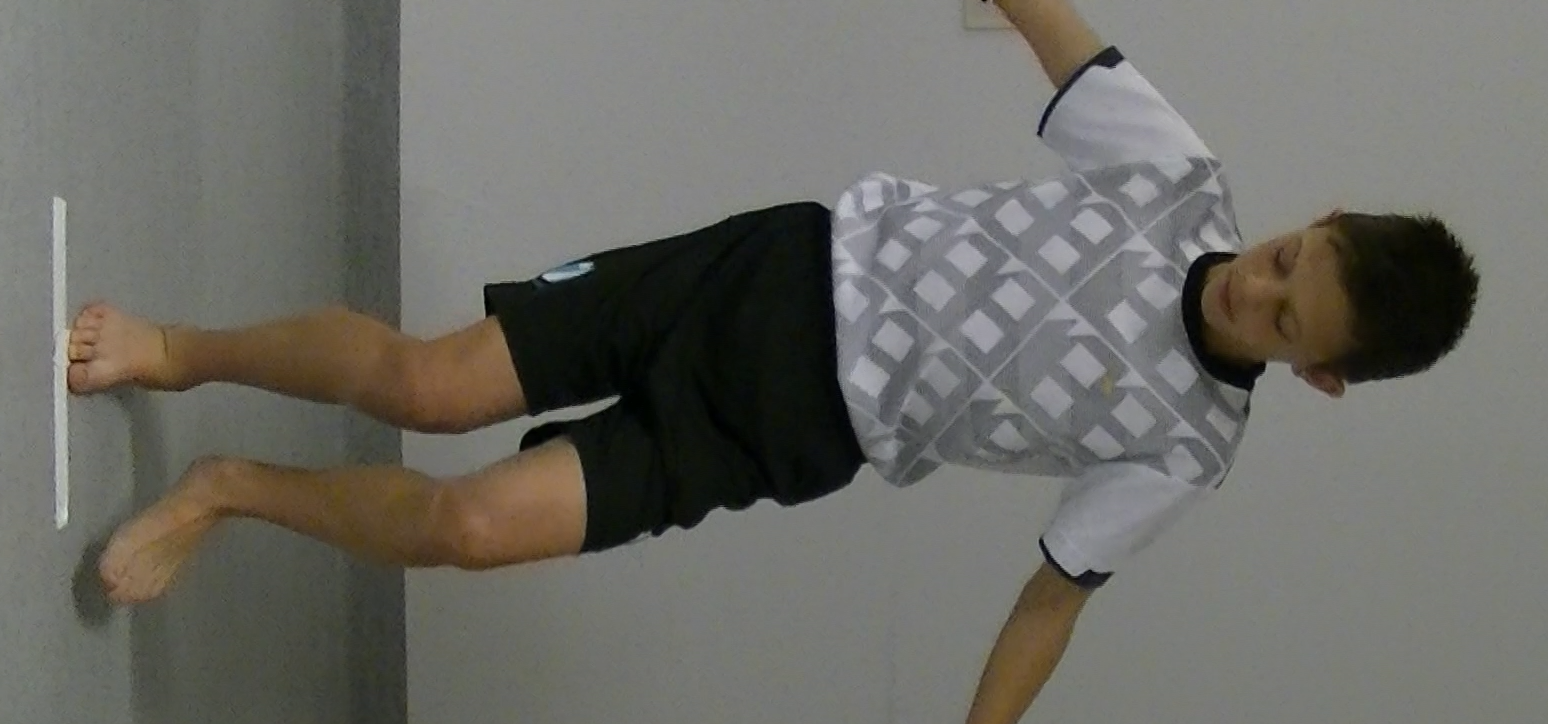
\includegraphics[angle=90,height=0.7\textheight]{files/figs/presentation/poor-poe.png}
        % \caption{}
        % \label{}
      \end{figure}
  \end{columns}
  % \vspace{0.1cm}
  {\scriptsize\textbf{Figure 2:} Examples of maintained (left) and altered postural orientation (right) during a single leg squat. \newline}
  \column{0.45\textwidth}
  \begin{itemize}
    \item Ability to uphold alignment of body parts.
    \item Altered PO - seen to increase risk of re-injury.
    \item No established and feasible method to assess for clinical use.
    \item When used, found from motion capture systems.
    % \item Proposed methods where experts assess motions on videos - time consuming\footnotemark.
  \end{itemize}
  \end{columns}

  % \footnotetext[10]{\hspace Nae et al., Extended Version of a Test Battery for Visual Assessment of Postural Orientation Errors: Face Validity, Internal Consistency, and Reliability. 2020}

  % \begin{figure}
  %   \centering
  %   \begin{subfigure}[t]{0.45/textwidth}
  %       \raggedleft
  %       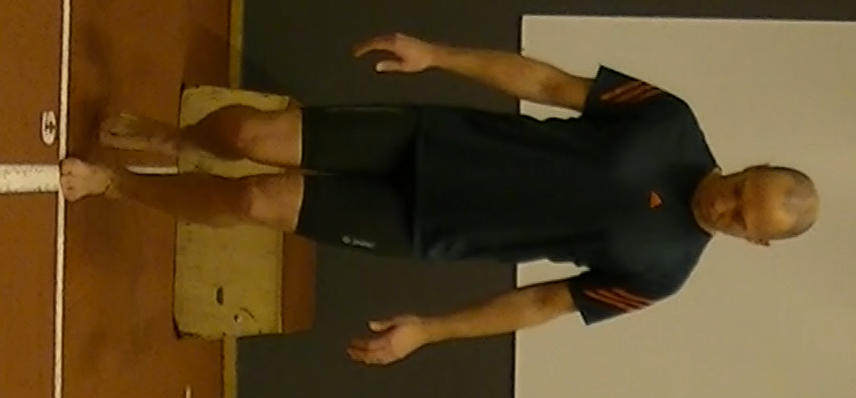
\includegraphics[height=0.5\textheight,angle=90]{files/figs/presentation/good-poe.png}
  %   \end{subfigure}
  %   ~
  %   \begin{subfigure}[t]{0.45\textwidth}
  %     \raggedright
  %     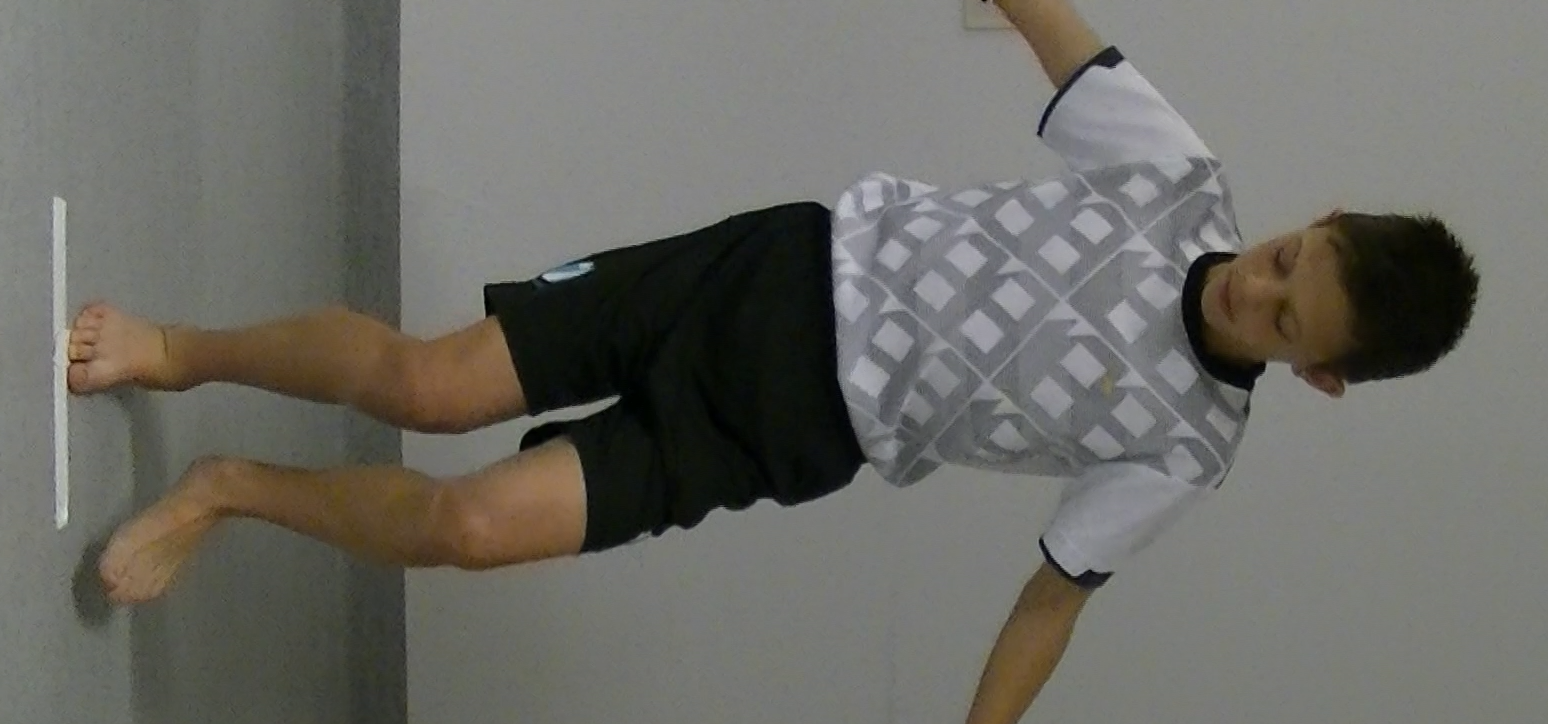
\includegraphics[height=0.5\textheight,angle=90]{files/figs/presentation/poor-poe.png}
  %   \end{subfigure}
    % 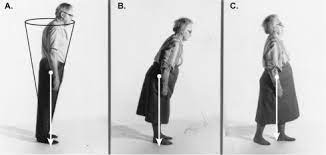
\includegraphics[height=0.5\textheight]{files/figs/presentation/postural-orientation.jpeg}
    %
    % {\scriptsize\textbf{Figure 3:} Examples of postural orientation\footnotemark}
    % \caption{}
    % \label{}
  % \end{figure}

% \footnotetext[10]{Horak, Postural orientation and equilibrium: what do we need to know about neural control of balance to prevent falls?. 2006}
\end{frame}

\begin{frame}[fragile]{Postural Orientation Errors in this work}
  \begin{columns}[T,onlytextwidth]
    \column{0.6\textwidth}
    \raggedleft
    % \begin{columns}[T,onlytextwidth]
    %   \column{0.03\textwidth}
    %
    %   \column{0.9\textwidth}
      \raggedright
      \vspace{0.3cm}
      \begin{itemize}
        \item Proposed methods where experts assess motions from videos\footnotemark.
        \item Scoring on ordinal scale, 0 (Good) - 2 (Poor).
        \item Patient score calculated as median of 4-5 repetition scores.
        \item Assessments are time consuming, can they be automated?
        % \item 6 different POEs for 5 different motions.
        \item Trunk, Pelvis, Femoral valgus, and KMFP POEs evaluated in this work for Single leg squat.
      \end{itemize}

    % \end{columns}

    \column{0.4\textwidth}
    \begin{figure}
      % \raggedleft
      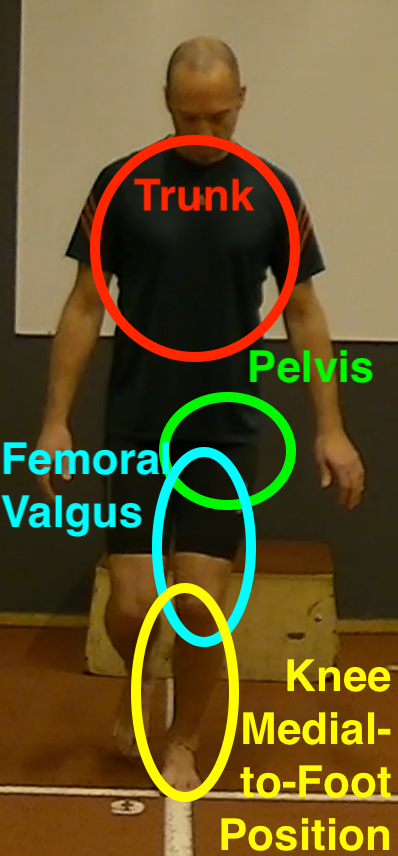
\includegraphics[height=0.76\textheight]{files/figs/presentation/poe-segments.png}

      {\scriptsize \hspace{0.5cm}\textbf{Figure 3:} Evaluated POEs.\newline}
    \end{figure}


      % \column{0.4\textwidth}
      % \begin{figure}
      %   \raggedleft
      %   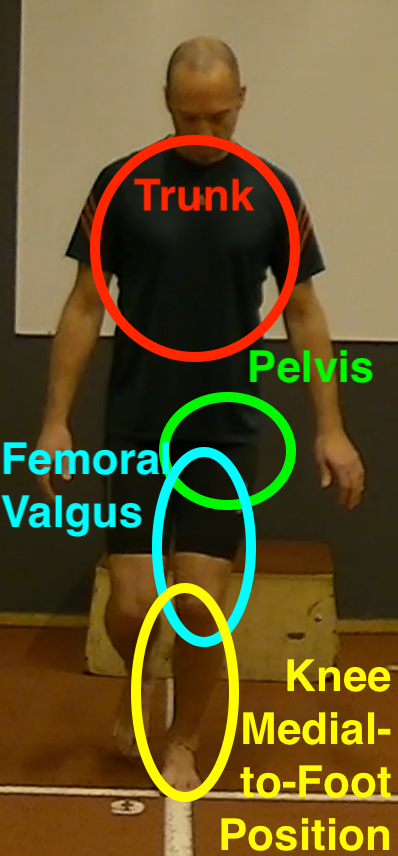
\includegraphics[height=0.76\textheight]{files/figs/presentation/poe-segments.png}
      %
      %   {\raggedleft\scriptsize \hspace{1cm}\textbf{Figure 4:} Evaluated POEs.\newline}
      %
      % \end{figure}
      %
      % \column{0.45\textwidth}
      % \raggedleft
      % \begin{itemize}
      %   \item Proposed methods where experts assess motions from videos\footnotemark.
      %   \item 6 different POEs for 5 different motions.
      %   \item Trunk, Pelvis, Femoral valgus, and KMFP POEs evaluated in this work for Single leg squat.
      % \end{itemize}
  \end{columns}

  \footnotetext[2]{\hspace Nae et al., Extended Version of a Test Battery for Visual Assessment of Postural Orientation Errors: Face Validity, Internal Consistency, and Reliability. 2020}
\end{frame}

\section{Methods}

\begin{frame}[fragile]{System overview}
    \begin{figure}
      \centering
      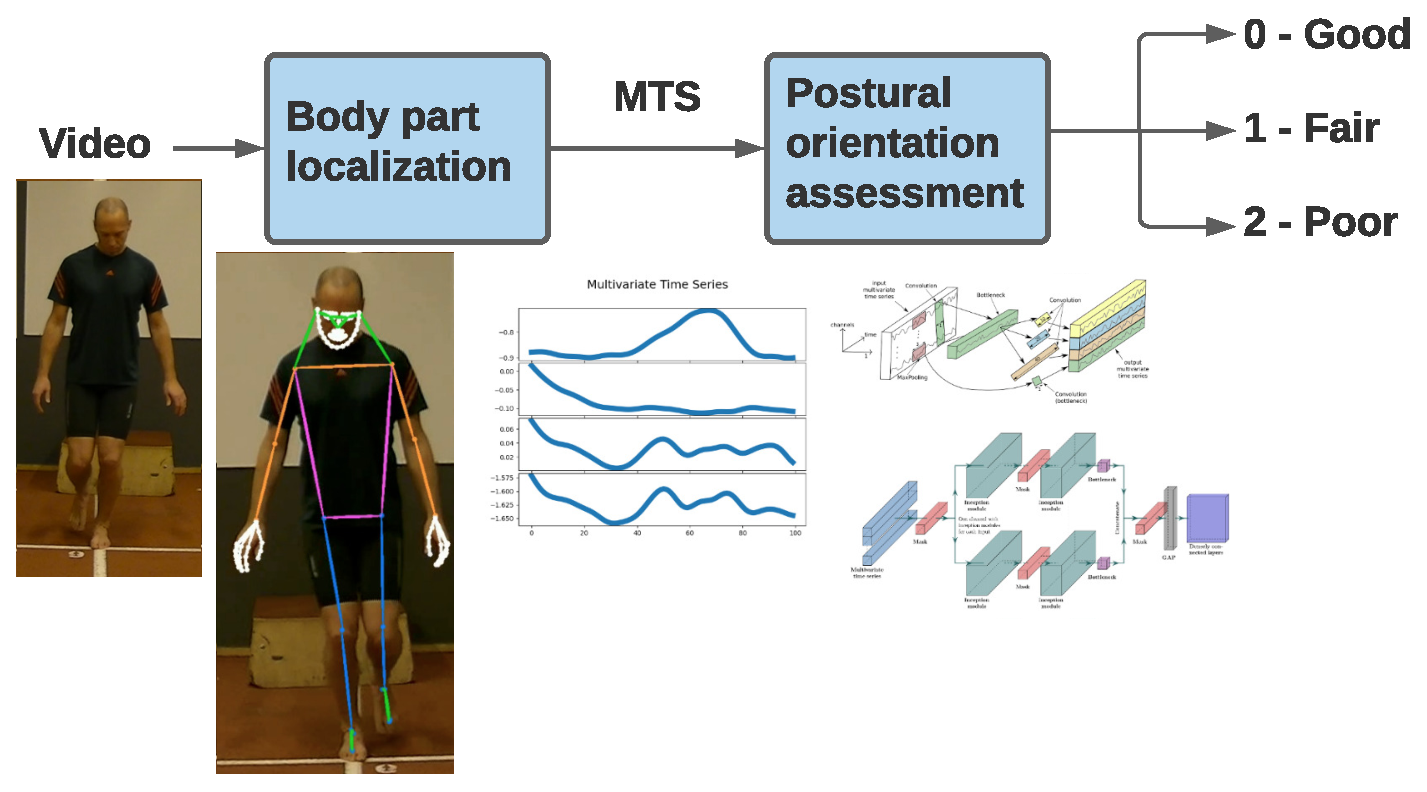
\includegraphics[width=\textwidth]{files/figs/presentation/sys-overview.eps}

      {\scriptsize\textbf{Figure 4:} POE assessment system overview.}
      % \caption{}
      % \label{}
    \end{figure}
\end{frame}

\begin{frame}[fragile]{Body part localization}
  \begin{columns}[T,onlytextwidth]
      \column{0.45\textwidth}
      % \animategraphics[loop,controls={play,stop},height=0.7\textheight]{25}{files/figs/presentation/sls06-pngs/sls06L-imgs-}{0}{539}

      % embedda video pa ngt satt

      \column{0.55\textwidth}
      \begin{itemize}
        \item Built upon MMPose framework\footnotemark.
        \item HRNet\footnotemark with DARK-pose\footnotemark trained on COCO-wholebody dataset used for pose estimation.
        \item Outputs 133 keypoint coordinates.
      \end{itemize}
  \end{columns}

  \footnotetext[3]{MMPose - OpenMMLab, \url{https://github.com/open-mmlab/mmpose}}
  \footnotetext[4]{Sun et al., Deep high-resolution representation learning for human pose estimation. 2019}
  \footnotetext[5]{Zhang et al., Distribution-Aware Coordinate Representation for Human Pose Estimation. 2020}


  % \movie[height=\textheight,poster]{}{files/figs/presentation/06-SLS-L-25.mp4}
\end{frame}
% prata om hur pixel space reduceras till keypoint space,
%

\begin{frame}[fragile]{Time series classification - Network architectures}
  \begin{columns}[c,onlytextwidth]
    \column{0.55\textwidth}
    \begin{figure}
      \centering
      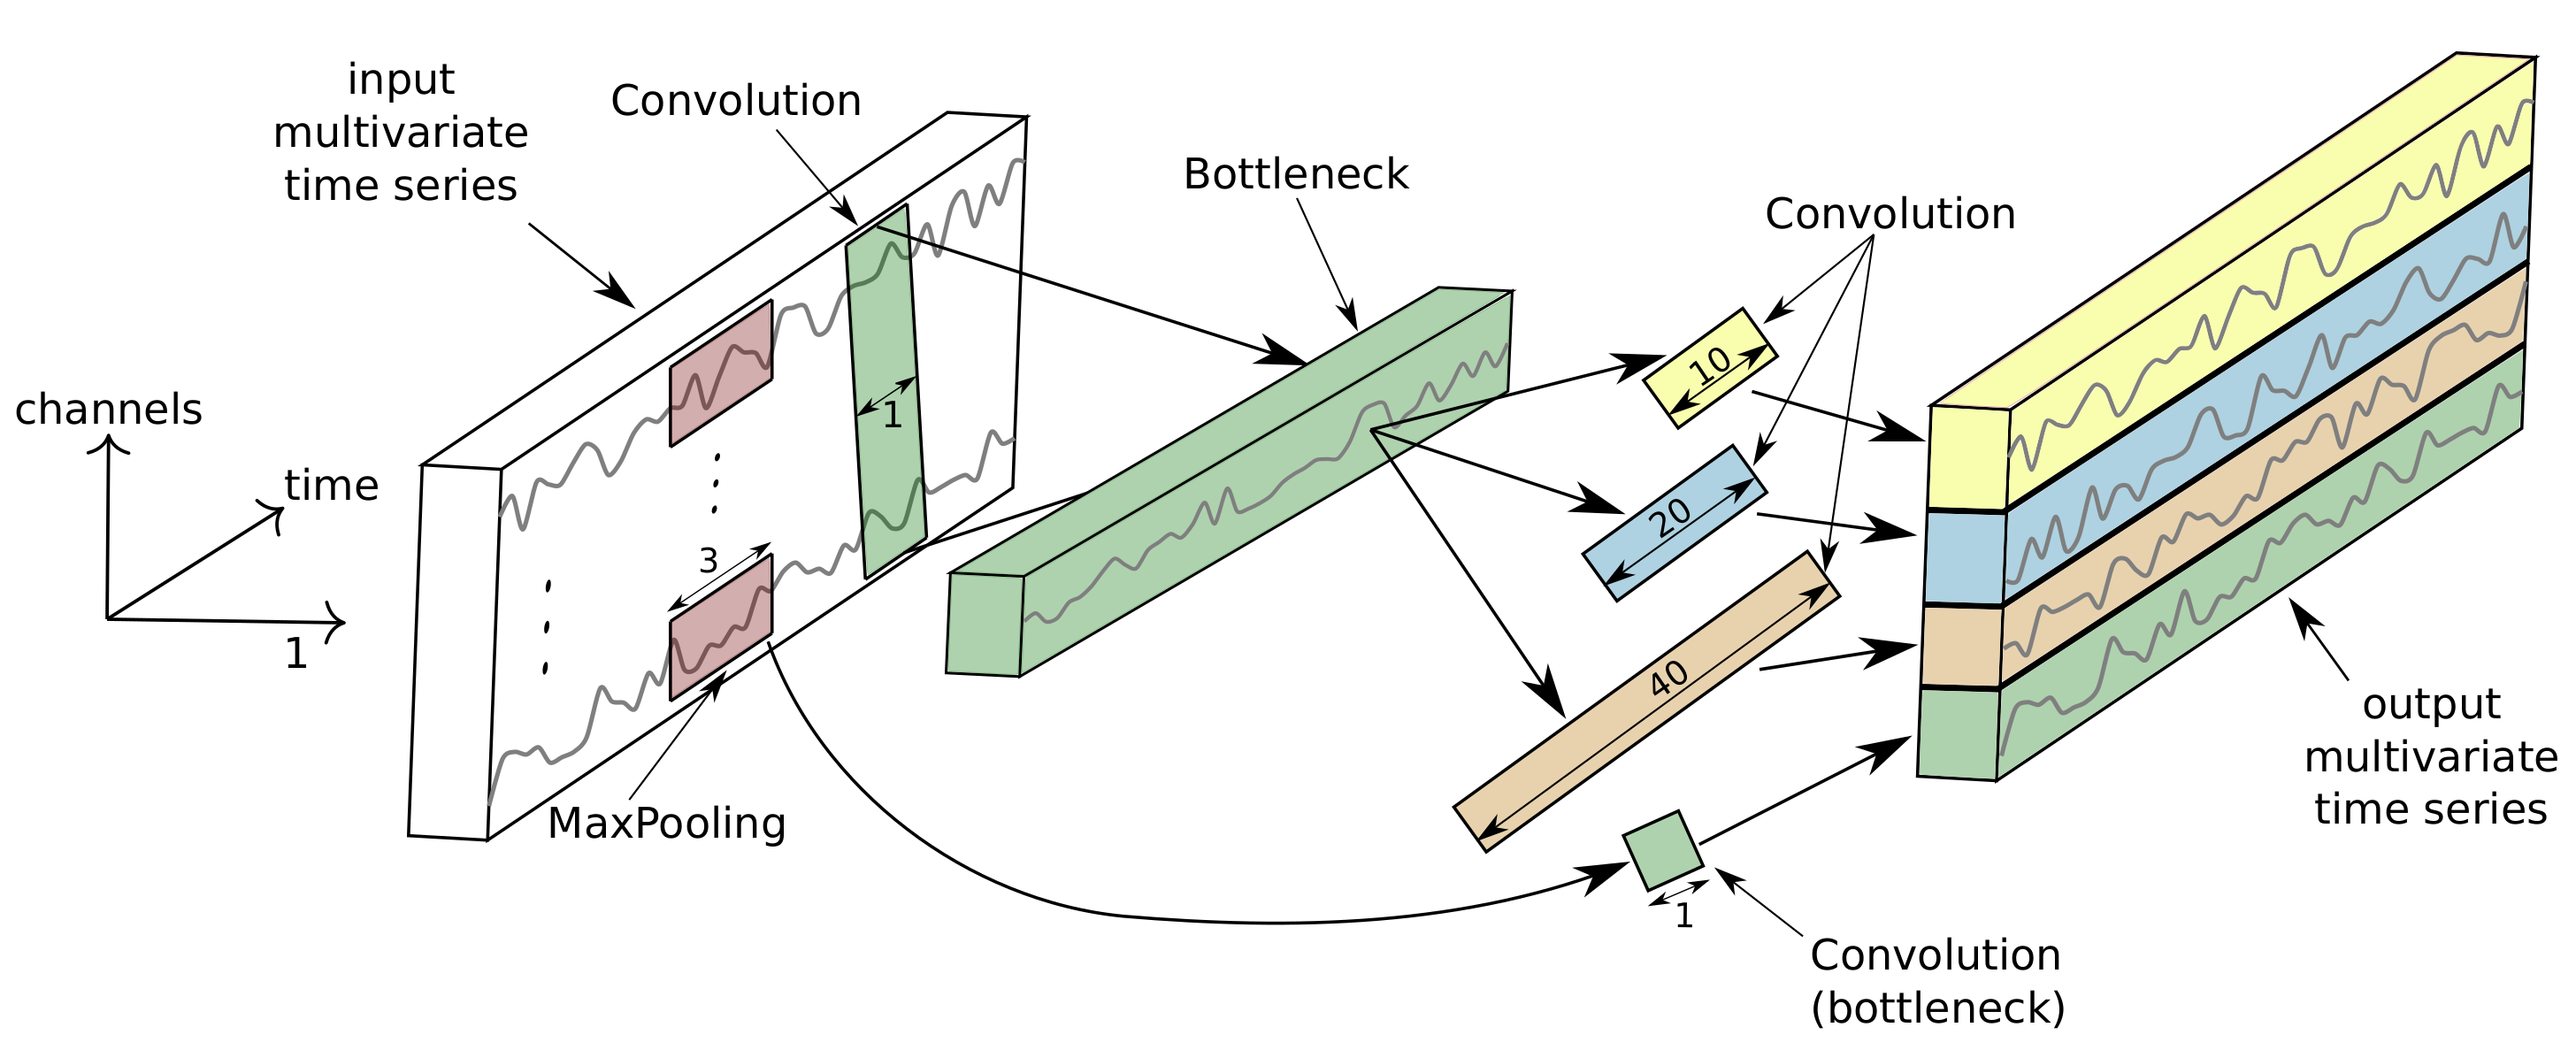
\includegraphics[width=\textwidth]{files/figs/tsc/inception-time-module.png}
      {\scriptsize\textbf{Figure 5:} InceptionTime module$^6$.}
      % \caption{}
      % \label{}
    \end{figure}

  \column{0.4\textwidth}
  \begin{block}{IncetionTime\footnotemark}
    Modules with convolutions of different lengths, global average pooling, and densely connected layers for classification.
  \end{block}
  \end{columns}

  \begin{columns}[c,onlytextwidth]
    \column{0.55\textwidth}
    \begin{figure}
      \centering
      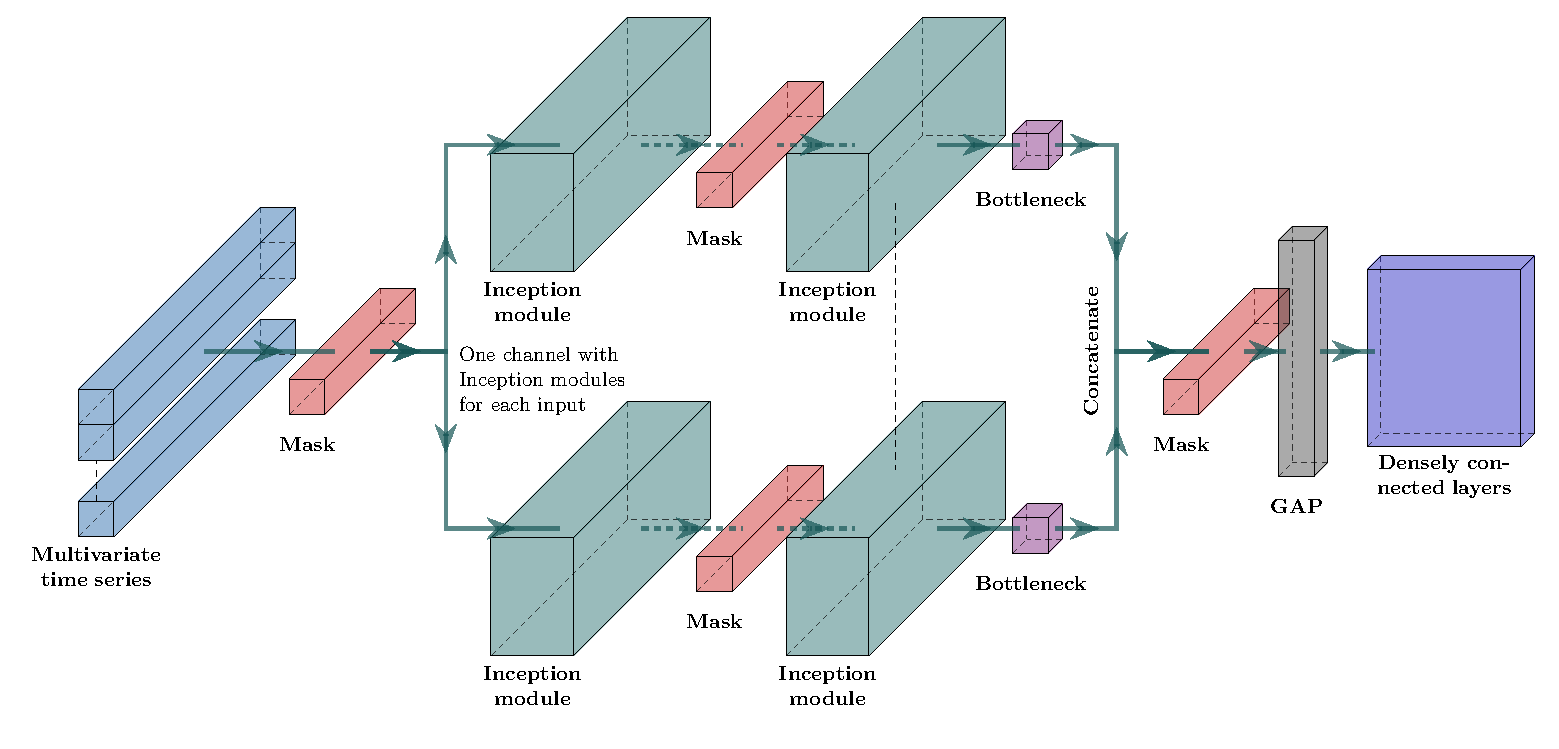
\includegraphics[width=\textwidth]{files/figs/met/x-inception-w-masks.pdf}
      {\scriptsize\textbf{Figure 6:} X-InceptionTime.}
      % \caption{}
      % \label{}
    \end{figure}

  \column{0.4\textwidth}
  \begin{block}{X-IncetionTime}
    Like InceptionTime, but input channels are kept separate.
  \end{block}
  \end{columns}

\footnotetext[6]{Fawaz et al., InceptionTime: Finding AlexNet for time series classification. 2020}
\end{frame}

\begin{frame}[fragile]{Inputs to classification}
  \begin{columns}
    \column{\dimexpr\paperwidth-20pt}
  \begin{table}
    % \caption{Inputs to the models classifying the different POEs. If the task was performed with the left leg the video has been mirrored, as described in Section \ref{sec:met-loc}.}
    % \label{tab:model-inputs}
    \caption{Input variables for the different POEs. Videos have been mirrored such that action is performed with right leg, if applicable.}
      \begin{center}
          \tabulinesep=0.8mm
          \begin{minipage}[t]{0.25\textwidth}
            \begin{tabu}[t]{l}
              \small
              \textbf{Trunk} \\ \hline \hline
              Left shoulder - $x$\\
              Right shoulder - $x$\\
              Right shoulder - $y$\\
              Left hip - $x$\\
              Left hip - $y$\\
              Right hip - $x$\\
              \multicolumn{1}{l}{\begin{tabular}[l]{@{}l@{}}Difference: right\\ hip and knee - $x$\end{tabular}}
            \end{tabu}
          \end{minipage}%
          \begin{minipage}[t]{0.25\textwidth}
            \begin{tabu}[t]{l}
              \small
              \textbf{Pelvis} \\ \hline \hline
              Right shoulder - $x$\\
              Right shoulder - $y$\\
              Right hip - $x$\\
              Right hip - $y$\\
              Left hip - $y$\\
              \multicolumn{1}{l}{\begin{tabular}[l]{@{}l@{}}Difference: right\\ hip and knee - $x$\end{tabular}}\\
              \multicolumn{1}{l}{\begin{tabular}[l]{@{}l@{}}Difference: right\\ knee and toes - $x$\end{tabular}}
            \end{tabu}
          \end{minipage}%
          \begin{minipage}[t]{0.24\textwidth}
            \begin{tabu}[t]{l}
              \small
              \textbf{Femoral Valgus} \\ \hline \hline
              Right shoulder - $x$\\
              Right hip - $x$\\
              Right knee - $y$\\
              \multicolumn{1}{l}{\begin{tabular}[l]{@{}l@{}}Angle: right\\ knee and ankle\end{tabular}}
            \end{tabu}
          \end{minipage}%
          \begin{minipage}[t]{0.25\textwidth}
            \begin{tabu}[t]{l}
              \small
              \textbf{KMFP} \\ \hline \hline
              Left shoulder - $y$\\
              Right hip - $y$\\
              \multicolumn{1}{l}{\begin{tabular}[l]{@{}l@{}}Angle: right\\ ankle and toes\end{tabular}}\\
              \multicolumn{1}{l}{\begin{tabular}[l]{@{}l@{}}Difference: right\\ hip and knee - $x$\end{tabular}} \\
              \multicolumn{1}{l}{\begin{tabular}[l]{@{}l@{}}Difference: right\\ knee and ankle - $x$\end{tabular}}
              % \multicolumn{1}{l}{\begin{tabular}[l]{@{}l@{}}Difference: right\\ knee and ankle - $x$\end{tabular}}
            \end{tabu}
          \end{minipage}%
      \end{center}
  \end{table}
  \end{columns}
\end{frame}

\begin{frame}[fragile]{Time series classification - Ensembles}
\begin{columns}[onlytextwidth]
\column{0.5\textwidth}
\begin{itemize}
  \item Each classification is obtained from ensembles of 5 classifier models.
  \item 2 models perform well over all classes - CORAL\footnotemark ordinal classifiers.
  \item Remaining models optimized for low false positive rates for one class each - class weights or modified cross-entropy loss.
\end{itemize}

\column{0.45\textwidth}
\begin{figure}
  \centering
  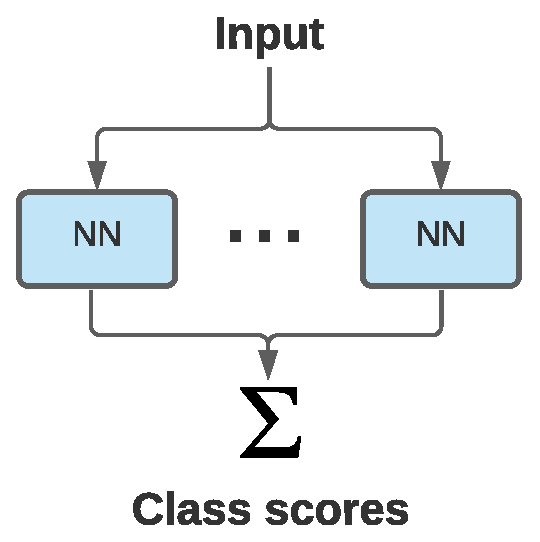
\includegraphics[width=\textwidth]{files/figs/presentation/ensemble.eps}
\end{figure}
{\scriptsize\newline\textbf{Figure 7:} Ensemble struture used for classification.}
\end{columns}
  % prata om fem modeller/poe. 2 almanna, med coral ordinal (presentera denna lite), och tre high precision models (presentera den loss function??)
  %
  % ngt mer ??

  \footnotetext[7]{Cao et al., Rank consistent ordinal regression for neural networks with application to age estimation. 2019}
  \end{frame}

\end{frame}

% \begin{frame}[fragile]{Combined score}
%
% \end{frame}
\section{Results}
\begin{frame}[fragile]{Data}
  % beskriv datan, typ video/reps, Antal, training/test split. Cross-val
  \begin{columns}[c]
    \column{0.55\textwidth}
    \begin{columns}
      \centering
      \column{0.6\textwidth}
      \begin{figure}
        \centering
        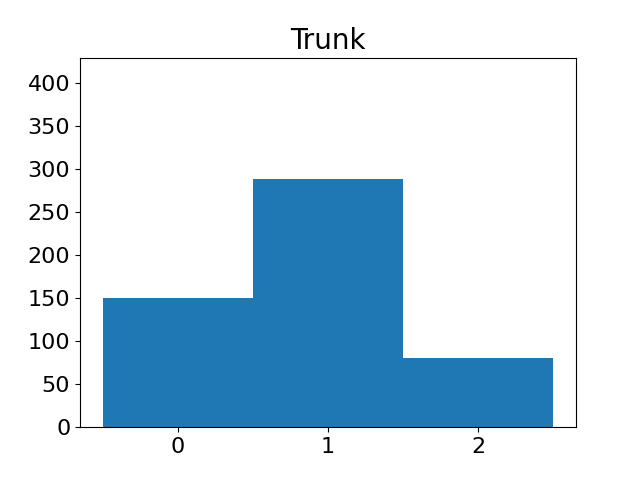
\includegraphics[width=\textwidth]{files/figs/met/trunk-label-hist.png}
        % \caption{}
        % \label{}
      \end{figure}

      \begin{figure}
        \centering
        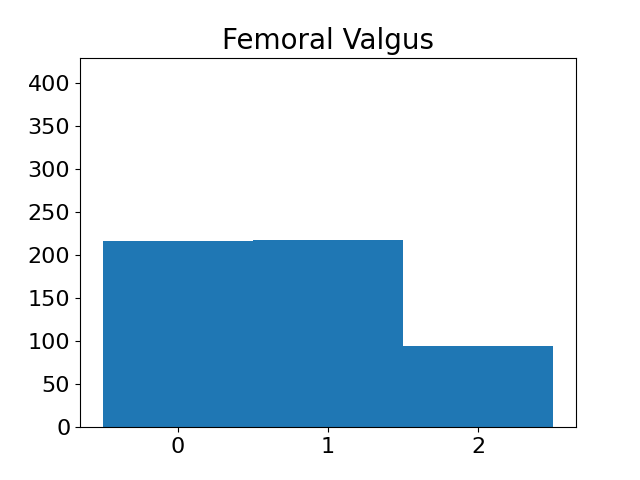
\includegraphics[width=\textwidth]{files/figs/met/femval-label-hist.png}
        % \caption{}
        % \label{}
      \end{figure}

      \column{0.6\textwidth}
      \begin{figure}
        \centering
        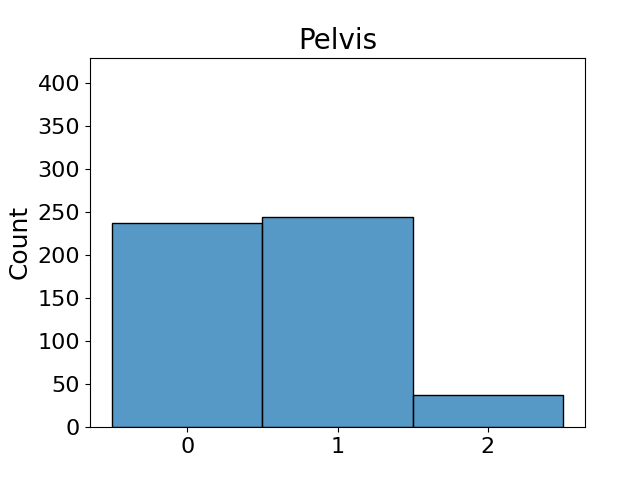
\includegraphics[width=\textwidth]{files/figs/met/pelvis-label-hist.png}
        % \caption{}
        % \label{}
      \end{figure}

      \begin{figure}
        \centering
        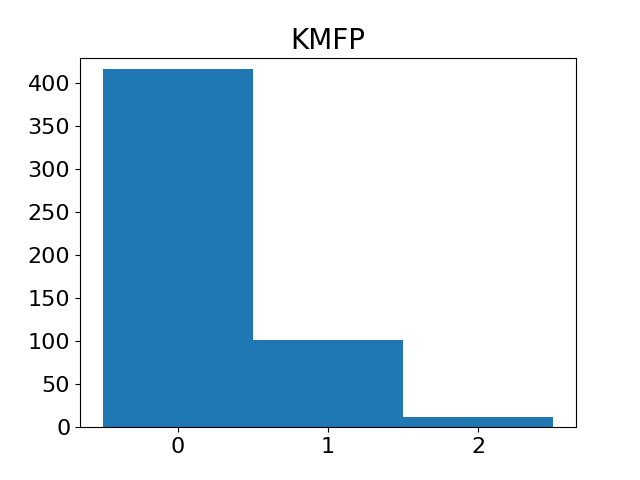
\includegraphics[width=\textwidth]{files/figs/met/kmfp-label-hist.png}
        % \caption{}
        % \label{}
      \end{figure}
    \end{columns}

    {\scriptsize\newline\textbf{Figure 8:} Class distributions for the different POEs.}

    \column{0.45\textwidth}
    \begin{itemize}
      \small
      \item Videos with 4-5 repetitions.
      \item 103 unique subjects.
      \item Assessments for right and left leg for some subjects/POEs - 105-107 assessed videos, 519-530 repetitions.
      \item 20\% (22 unique subjects, 110 repetitions) test set.
      \item 10-fold cross-validation used. Results shown are mean ($\pm$ std) of the 10 resulting models on test set.
    \end{itemize}

  \end{columns}
\end{frame}

\begin{frame}[fragile]{Trunk}
  \begin{columns}
    \column{0.5\textwidth}
    \textbf{\small~Accuracy (\%):} 73.7$\pm$4.5
    \vspace{0.3cm}
    \column{0.5\textwidth}
    \centering
    75.0$\pm$7.9
    \vspace{0.3cm}
  \end{columns}
  \begin{columns}
    \column{0.5\textwidth}
    \centering
    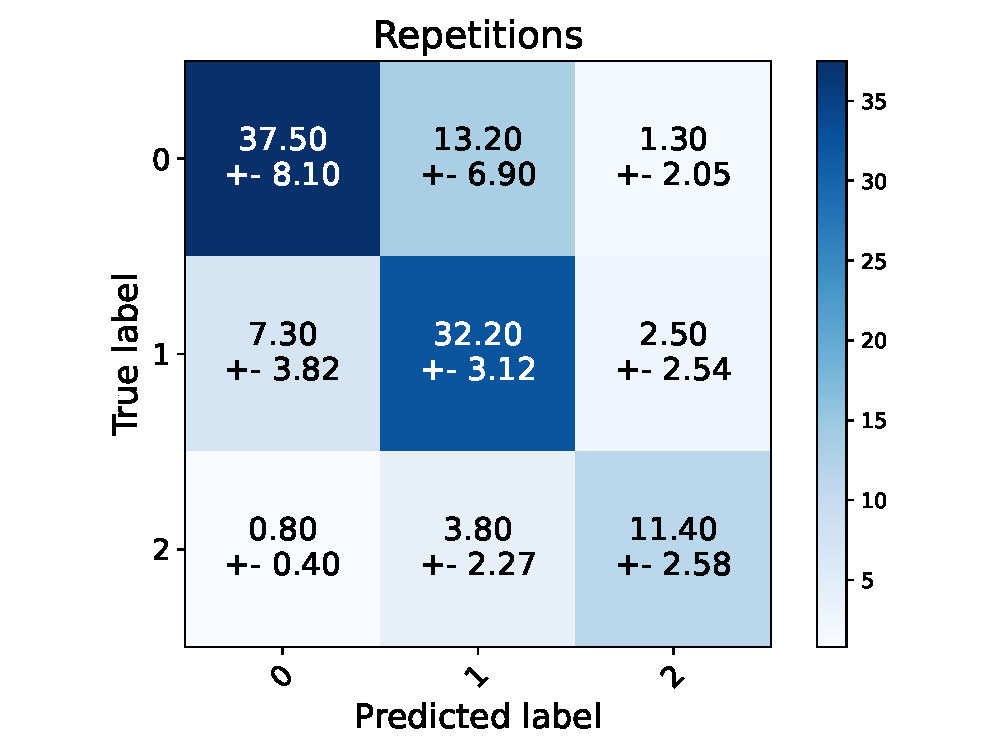
\includegraphics[width=\textwidth]{files/figs/res/trunk/cnf-reps.eps}
    \column{0.5\textwidth}
    \centering
    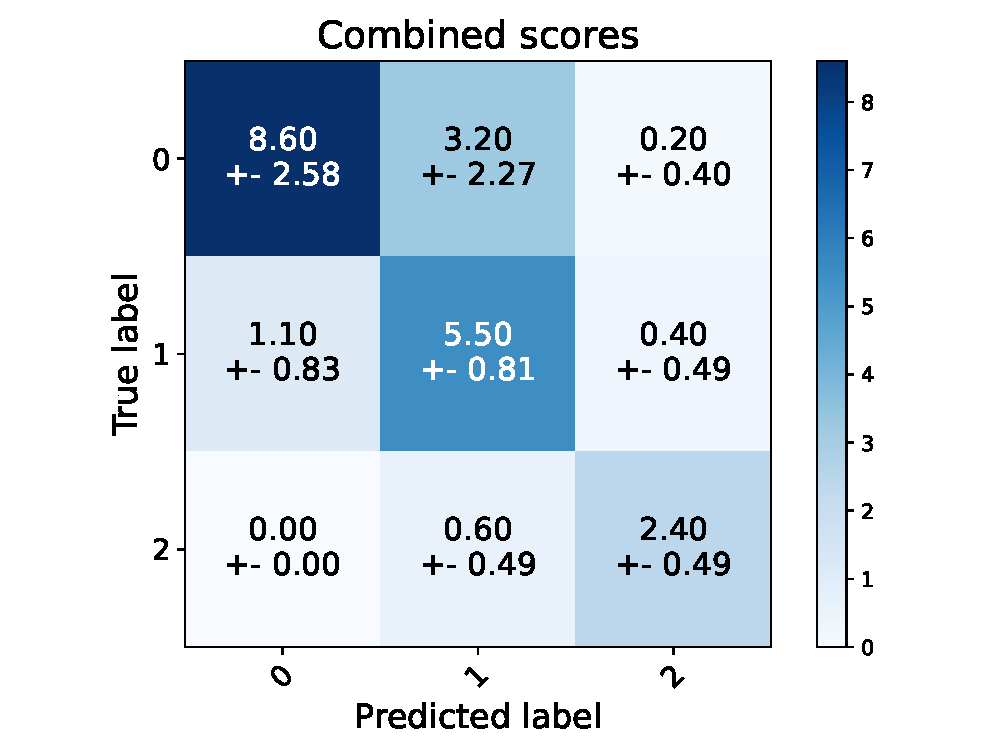
\includegraphics[width=\textwidth]{files/figs/res/trunk/cnf-combined.eps}
  \end{columns}
  % {\scriptsize\newline\textbf{Figure 10:} Confusion matrices for the classification of the repetitions (left) and the combined scores with thresholds ignoring uncertain predictions (right).}
  {\scriptsize\newline\textbf{Figure 9:} Confusion matrices for the classification of the repetitions (left) and the combined scores (right).}
\end{frame}

\begin{frame}[fragile]{Pelvis}
  \begin{columns}
    \column{0.5\textwidth}
    \textbf{\small~Accuracy (\%):} 63.6$\pm$10.7
    \vspace{0.3cm}
    \column{0.5\textwidth}
    \centering
    69.1$\pm$10.1
    \vspace{0.3cm}
  \end{columns}
  \begin{columns}
    \column{0.5\textwidth}
    \centering
    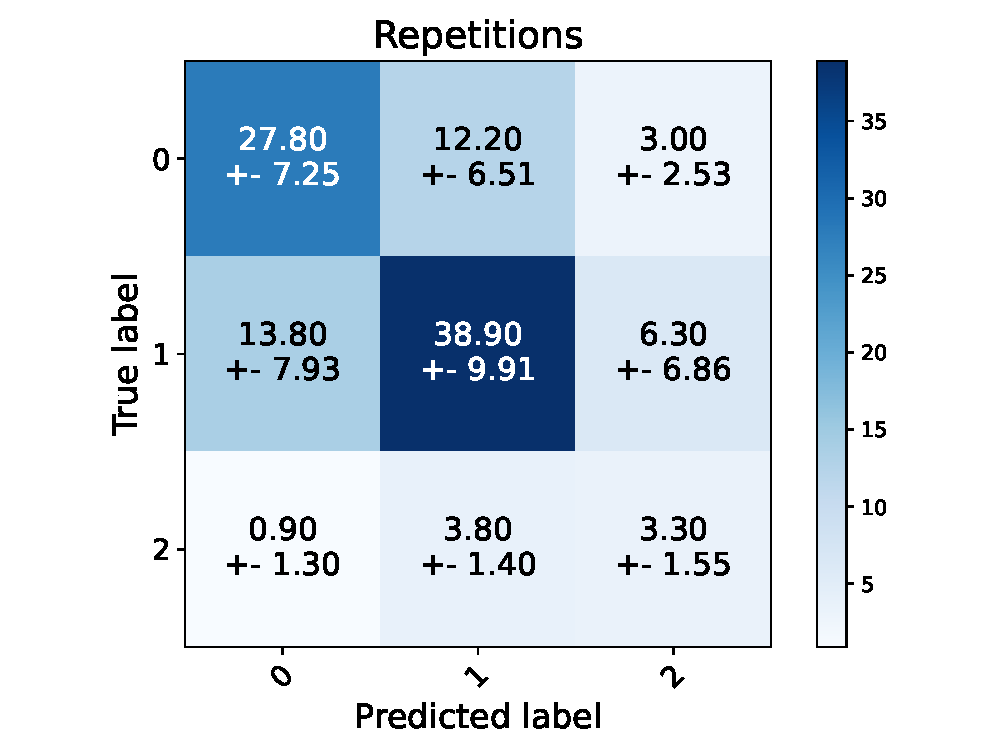
\includegraphics[width=\textwidth]{files/figs/res/pelvis/cnf-reps.eps}
    \column{0.5\textwidth}
    \centering
    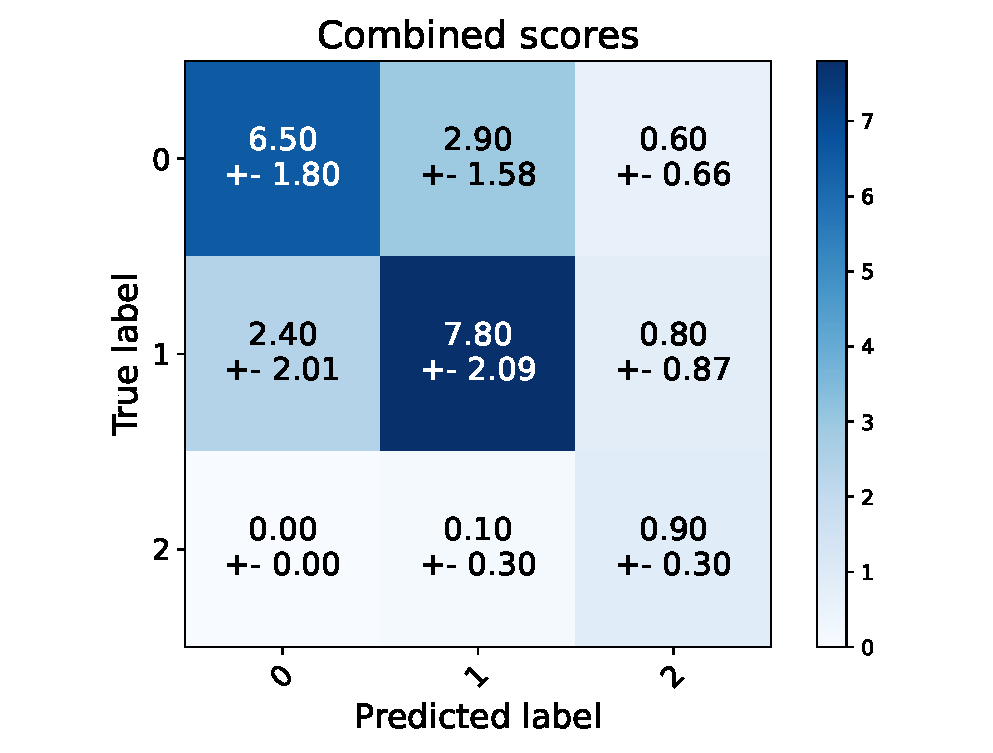
\includegraphics[width=\textwidth]{files/figs/res/pelvis/cnf-combined.eps}
  \end{columns}
  % {\scriptsize\newline\textbf{Figure 11:} Confusion matrices for the classification of the repetitions (left) and the combined scores with thresholds ignoring uncertain predictions (right).}
  {\scriptsize\newline\textbf{Figure 10:} Confusion matrices for the classification of the repetitions (left) and the combined scores (right).}
\end{frame}

\begin{frame}[fragile]{Femoral Valgus}
  \begin{columns}
    \column{0.5\textwidth}
    \textbf{\small~Accuracy (\%):} 69.6$\pm$6.8
    \vspace{0.3cm}
    \column{0.5\textwidth}
    \centering
    79.1$\pm$9.3
    \vspace{0.3cm}
  \end{columns}
  \begin{columns}
    \column{0.5\textwidth}
    \centering
    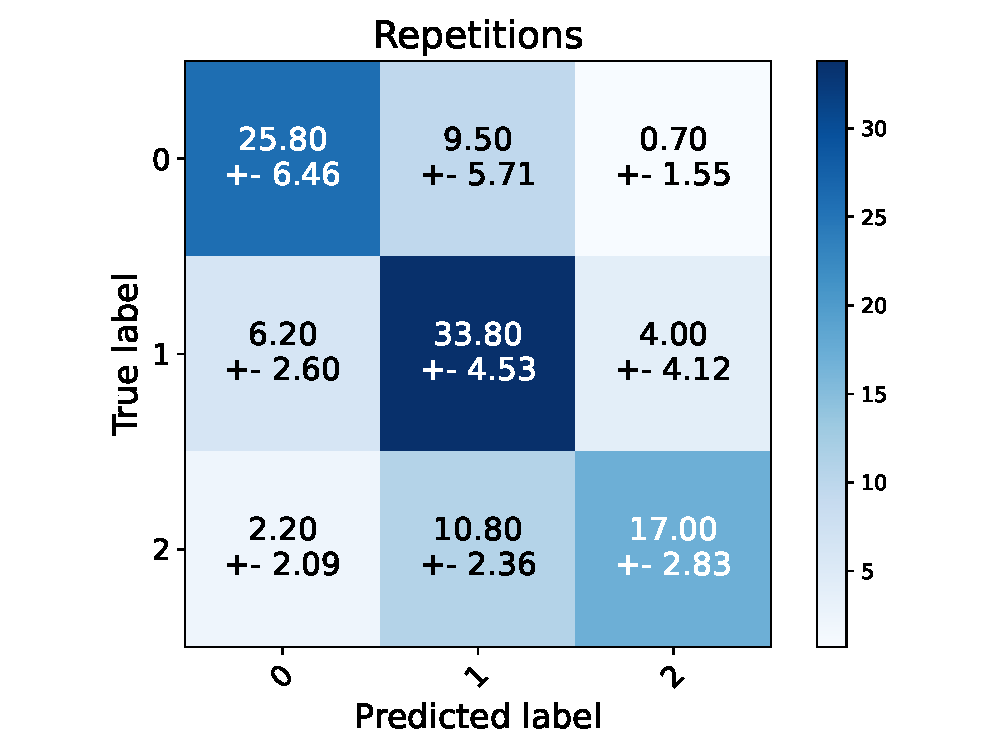
\includegraphics[width=\textwidth]{files/figs/res/femval/cnf-reps.eps}
    \column{0.5\textwidth}
    \centering
    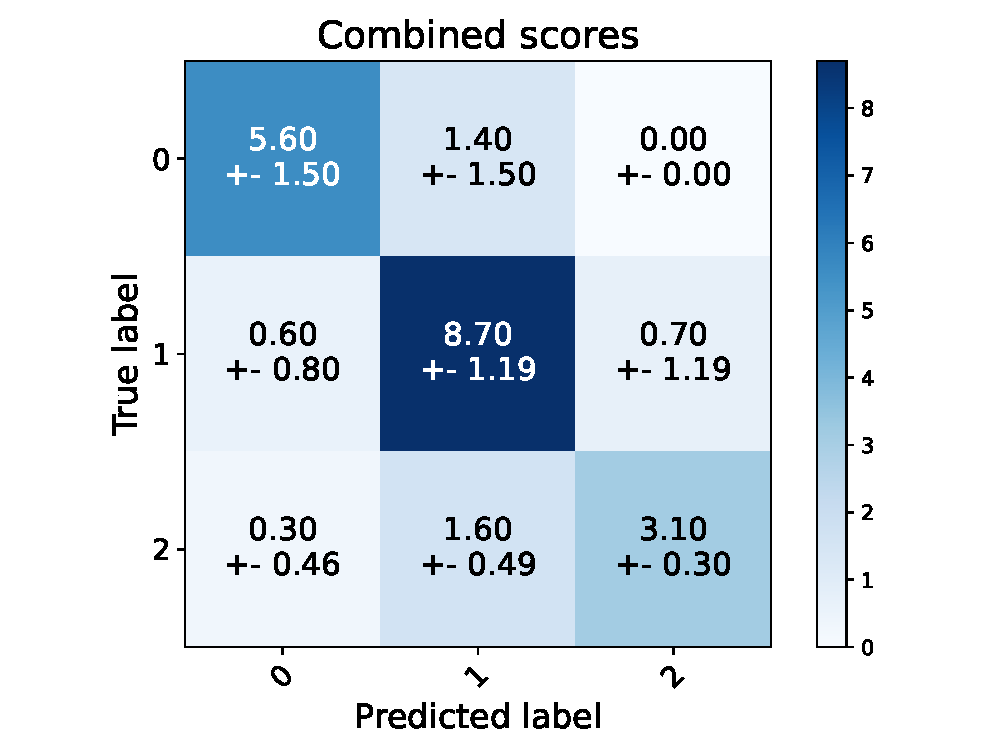
\includegraphics[width=\textwidth]{files/figs/res/femval/cnf-combined.eps}
  \end{columns}
  % {\scriptsize\newline\textbf{Figure 12:} Confusion matrices for the classification of the repetitions (left) and the combined scores with thresholds ignoring uncertain predictions (right).}
  {\scriptsize\newline\textbf{Figure 11:} Confusion matrices for the classification of the repetitions (left) and the combined scores (right).}
\end{frame}

\begin{frame}[fragile]{Knee Medial-to-Foot Position}
  \begin{columns}
    \column{0.5\textwidth}
    \textbf{\small~Accuracy (\%):} 82.3$\pm$3.1
    \vspace{0.3cm}
    \column{0.5\textwidth}
    \centering
    % 90.3$\pm$4.3
    89.5$\pm$4.5
    \vspace{0.3cm}
  \end{columns}
  \begin{columns}
    \column{0.5\textwidth}
    \centering
    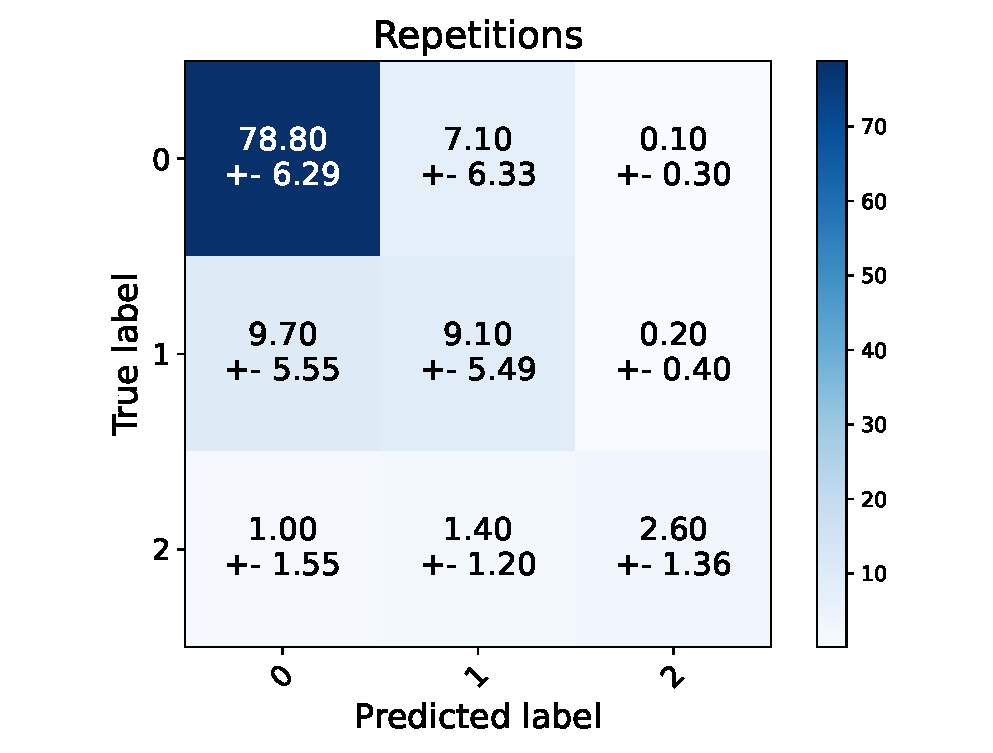
\includegraphics[width=\textwidth]{files/figs/res/kmfp/cnf-reps.eps}
    \column{0.5\textwidth}
    \centering
    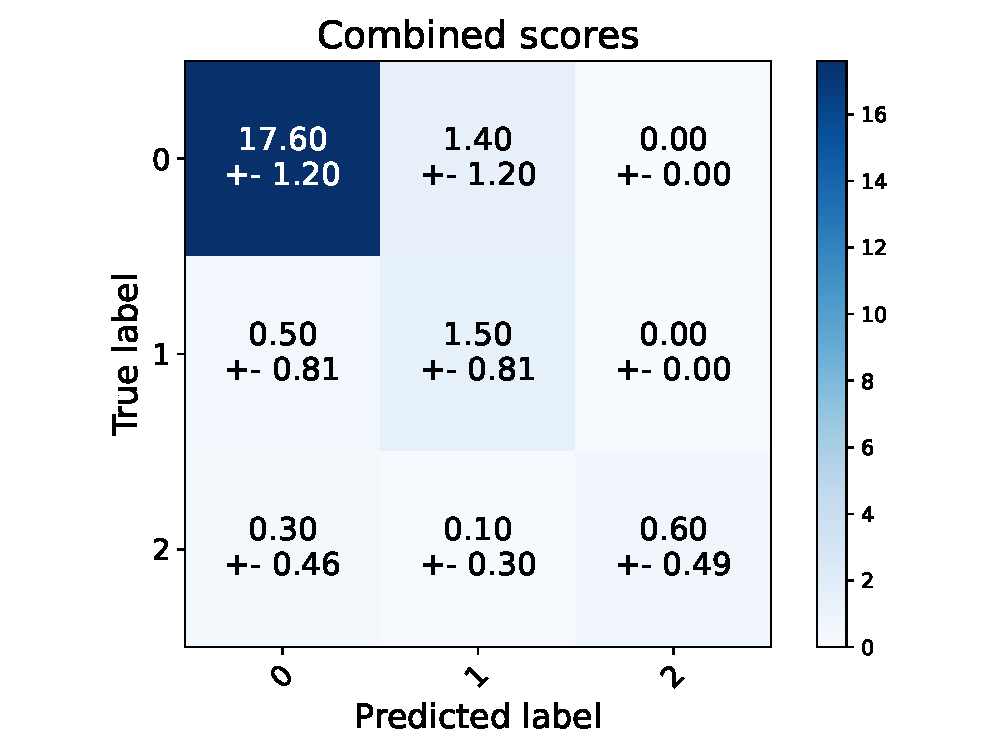
\includegraphics[width=\textwidth]{files/figs/res/kmfp/cnf-combined.eps}
  \end{columns}
  % {\scriptsize\newline\textbf{Figure 13:} Confusion matrices for the classification of the repetitions (left) and the combined scores with thresholds ignoring uncertain predictions (right).}
  {\scriptsize\newline\textbf{Figure 12:} Confusion matrices for the classification of the repetitions (left) and the combined scores (right).}
\end{frame}

\begin{frame}[fragile]{Summary}
  \begin{table}[h]
    % \caption{Approximative 95\% confidence intervals for the performance of the combined scores with thresholds for different POEs, assuming Gaussian distributions. }
    % \label{tab:sum-ci}
    \caption{Summary of results, here the combined sccores with thresholds removing samples the models are uncertain about.}
    \centering
    \begin{tabu}[c]{|c|c|c|c|c|}
      \hline
      & \textbf{Trunk} & \textbf{Pelvis} &\textbf{Femoral Valgus} & \textbf{KMFP} \\ \hline
      \textbf{Accuracy (\%)}  & 80.0$\pm$7.8 & 73.3$\pm$18.9 & 82.3$\pm$6.0 & 90.3$\pm$4.3 \\\hline
      \textbf{F1 score (\%)}  & 79.9$\pm$8.9 & 73.6$\pm$22.3 & 81.0$\pm$5.2 & 74.0$\pm$22.3 \\ \hline
      \textbf{Recall (\%)}    & 81.6$\pm$7.2 & 77.9$\pm$14.9  & 79.5$\pm$5.5 & 81.1$\pm$24.7 \\ \hline
      \textbf{Precision (\%)} & 83.0$\pm$6.8 & 74.9$\pm$23.8 & 86.5$\pm$5.6 & 71.4$\pm$22.6 \\\hline
      % & \textbf{Trunk} & \textbf{Pelvis} &\textbf{Femoral Valgus} & \textbf{KMFP} \\ \hline
      % \textbf{Accuracy (\%)}  & 80.0$\pm$4.9 & 73.3$\pm$11.9 & 82.3$\pm$3.8 & 90.3$\pm$2.7 \\\hline
      % \textbf{F1 score (\%)}  & 79.9$\pm$5.6 & 73.6$\pm$14.1 & 81.0$\pm$3.3 & 74.0$\pm$14.1 \\ \hline
      % \textbf{Recall (\%)}    & 81.6$\pm$4.6 & 77.9$\pm$9.4  & 79.5$\pm$3.5 & 81.1$\pm$15.6 \\ \hline
      % \textbf{Precision (\%)} & 83.0$\pm$4.3 & 74.9$\pm$15.1 & 86.5$\pm$3.5 & 71.4$\pm$14.3 \\\hline
    \end{tabu}
  \end{table}
\end{frame}

\section{Conclusions and Future work}

\begin{frame}[fragile]{Conclusions and Future work}
  \begin{itemize}
    \item The results suggests the proposed method could automate assessments.
    \item Large variance in results suggests more data needed.
    \item Future work:
          \begin{itemize}
            \item Multiple experts to assess videos.
            \item Assess videos repetition-wise.
            \item Evaluate 3D coordinate reconstruction.
            \item Non-uniform weighting in ensembles and when combining scores.
            \item Assess more POEs and motions.
          \end{itemize}
  \end{itemize}

\end{frame}

\begin{frame}[standout]
  Thank you
\end{frame}

\appendix

\begin{frame}[fragile]{Backup slides}
  Sometimes, it is useful to add slides at the end of your presentation to
  refer to during audience questions.

  The best way to do this is to include the \verb|appendixnumberbeamer|
  package in your preamble and call \verb|\appendix| before your backup slides.

  \themename will automatically turn off slide numbering and progress bars for
  slides in the appendix.
\end{frame}



\end{document}
